\subsection{Shirley Temple}
\vspace{-7.4mm}
\hspace{42mm}
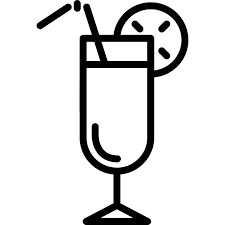
\includegraphics[scale=.07]{cocktail_glass_tall.png}
\vspace{2.5mm}
\begin{itembox}[l]{\boldmath $\reci$}
\begin{itemize}
\setlength{\parskip}{0cm}
\setlength{\itemsep}{0cm}
\item \ga or \llsoda 130ml
\item \gs 20ml
\end{itemize}
\vspace{-4mm}
Garnish: \lemon or \lime 1-4cuts, \cherry 1-4\\
Made by \build
\end{itembox}
Sweet and refreshing, recommended to women and children.
It may have been invented by a bartender at Chasen's, a restaurant in West Hollywood, California, to serve then-child actress Shirley Temple.
Turns to Dirty Shirley by adding 45ml of \vodka or Rum.
